\documentclass[a4paper,12pt]{book}

\usepackage{apacite}
\usepackage{quotchap}
\usepackage{amssymb}
\usepackage{pdfpages}
\usepackage{pseudocode}
\usepackage{geometry}
\usepackage[english]{babel}
\usepackage{lscape}
\usepackage{graphicx}
\usepackage{appendix}
\usepackage{url}
\usepackage{framed}
\usepackage[framed]{ntheorem}
\usepackage{verbatim}
\usepackage{stmaryrd}
\usepackage{array}
\usepackage{caption}
\usepackage{subcaption}
\usepackage{vub}
\usepackage[T1]{fontenc}
%\usepackage[scaled]{uarial}
\usepackage{tocloft}
\renewcommand{\familydefault}{\sfdefault}
\usepackage{blindtext}
\usepackage{listings}
\usepackage{fancyhdr}

\definecolor{java}{RGB}{127,0,85}
\newcommand{\code}[1]{\texttt{#1}}
\lstset{language=Java, basicstyle=\scriptsize,breaklines=true, keywordstyle=\color{java},tabsize=1, frame=single}

\newcolumntype{C}[1]{>{\centering\let\newline\\\arraybackslash\hspace{0pt}}m{#1}}
\newcolumntype{L}[1]{>{\raggedright\let\newline\\\arraybackslash\hspace{0pt}}m{#1}}
\addtocontents{toc}{\cftpagenumbersoff{chapter}}

\newtheorem{hyp}{Hypothesis} 
\newframedtheorem{defshad}{Definition}
\newtheorem{defPim}{Definition}
\newframedtheorem{pilePrinc}{Principle}
\newframedtheorem{theo}{}
\newtheorem{req}{Requirement}

\setlength{\marginparwidth}{0pt}
\makeatletter
\renewcommand*{\sectfont}{\bfseries}
\renewcommand*{\chapnumfont}{%
  \usefont{T1}{\@defaultcnfont}{b}{n}\fontsize{120}{150}\selectfont% Default: 100/130
  \color{chaptergrey}%
}
\makeatother
\geometry{textwidth=390pt}

\geometry{bindingoffset=2cm}


\fancypagestyle{plain}{
  \fancyhf{}
  \fancyfoot[C]{}%
  \renewcommand{\headrulewidth}{0pt}% Line at the header invisible
}

\makeatletter
\renewcommand\paragraph{%
   \@startsection{paragraph}{4}{0mm}%
      {-\baselineskip}%
      {.5\baselineskip}%
      {\normalfont\normalsize\bfseries}}
\makeatother


\usepackage{amsmath}
\usepackage{bm}
\usepackage{svg}

\def\innerproduct{\langle\cdot _, \cdot\rangle}
\def\orthseq{\{ \varphi_n \}_{n=0}^\infty}

\author{Steven Homer}
\title{Learning Hierarchical Spectral \\
Representations of Human Speech \\
in the Information Dynamics of Thinking}
\promotortitle{Promoter}
\promotor{Prof. Dr. Dr. Geraint Wiggins}
\advisortitle{Advisor}                                                            
\advisors{Prof. Dr. Dr. Geraint Wiggins}
\faculty{Faculty of Science and Bio-engineering Sciences}
\department{Department of Computer Science}   
\subtitle{Graduation thesis submitted in partial fulfillment of the requirements for the degree of \\Master of Science in Applied Sciences and Engineering: Computer Science}
\date{Academic year 2018-2019}


\begin{document}
\pagestyle{fancy}
\setlength{\headheight}{14.5pt}
\renewcommand{\chaptermark}[1]{\markboth{\MakeUppercase{\chaptername}\ \thechapter.\ #1}{}}
\renewcommand{\sectionmark}[1]{\markright{#1}{}}
\fancyhf{}
\fancyhead[LO,RE]{\bfseries\thepage}
\fancyhead[RO]{\bfseries\leftmark}
\fancyhead[LE]{\bfseries\rightmark}
\renewcommand{\headrulewidth}{0.5pt}
% PARAGRAPH INDENTATION

%\setlength{\parskip}{0pt} % 1ex plus 0.5ex minus 0.2ex}
%\setlength{\parindent}{0pt}

\maketheses


\pagebreak
\setcounter{page}{1}
\pagenumbering{roman}

\section*{Abstract}

            
\newpage
\section*{Declaration of Originality}
I hereby declare that this thesis was entirely my own work and that any additional sources of information have been duly cited.
I certify that, to the best of my knowledge, my thesis does not infringe upon anyone's copyright nor violate any proprietary rights and that any ideas, techniques, quotations, or any other material from the work of other people included in my thesis, published or otherwise, are fully acknowledged in accordance with the standard referencing practices. Furthermore, to the extent that I have included copyrighted material, I certify that I have obtained a written permission from the copyright owner(s) to include such material(s) in my thesis and have included copies of such copyright clearances to my appendix. 
 
I declare that this thesis has not been submitted for a higher degree to any other University or Institution.

\newpage
\section*{Acknowledgements}

\newpage

\tableofcontents
\newpage
\listoffigures
\newpage
\listoftables
\newpage
\setcounter{page}{1}
\pagenumbering{arabic}
\newpage


\chapter{Introduction}
\include{tex/introduction/introduction}
\section{Context}

\section{Problems \& Justifications}

\section{Objectives \& Hypotheses}

\section{Research Method}

\section{Structure}


\chapter{Background}
\include{tex/background/background}
\section{Conceptual Spaces}
\label{section:conceptual-spaces}

In knowledge representation, the argument over the representation of cognition often falls into two camps: connectionism and symbolicism.  As the lowest level of represention, connectionism is best exemplified by artificial neural networks \citep{lecun2015deep}, where cognition emerges from myrid connections between neurons.  At the highest level, symbolicism views the mind as a Turing machine \citep{turing2009computing}, where cognition is equivalent to compution by symbol manipulation.  Conceptual spaces theory \citep{gardenfors2004conceptual} argues for a middle way, through the use of eponymous conceptual spaces.  Conceptual spaces theory views cognition as the process of concept formation by means of similarity, so that the continuous representations of connectionism can be bridged to the discrete representations of symbolicism, hopefully gaining the best of both worlds.  

Conceptual spaces theory states that representations in the mind are situated in conceptual spaces -- semantically rich spaces with geometric properties -- which allow for intuitive geometric reasoning about related objects. For instance, in the conceptual space of color with dimensions of hue, saturation, and brightness, one can formally make a geometric claim that “orange lies between yellow and red.”  This simple claim cannot be made by connectionism or symbolicism without imposing ad-hoc external semantics on the connection weights or symbols respectively, highlighting the explanatory power of conceptual spaces for knowledge representation.

\subsection{Quality Dimensions}
\label{section:quality-dimensions}

Quality dimensions are the basic building blocks of a conceptual space.  They can be thought of as the axes that give meaning to the elements in the space.  In three-dimensional Cartesian space, when referring to a point, we specify it by its placement on each of the $x$, $y$, and $z$ -axes.  By analogy, each of the $xyz$-axes would be a quality dimension in the 3D Cartesian space.  However, quality dimensions are more than just orthogonal unit vectors, they can also have their own specific geometry that serves to constrain the dimension. For instance, a quality dimension may have the geometry of a circle, resulting in different behavior than the real number line.  Quality dimensions also allow us to speak meaningfully about similarity between objects in a space since, by definition, they possess distance and betweenness relations.  Finally, it is important to remember that the 'quality' of the quality dimension is what gives it inherent semantic content beyond just being a descriptive dimension.

\subsection{Domains and Conceptual Spaces}
\label{section:domains-and-conceptual-spaces}

Integral quality dimensions require one another to exist.  For instance, the three qualities of sound: pitch, timbre, and loudness, are all integral to one another \citep{mcadams1985qualities}.  It is impossible to identify a sound without specifying all three of these dimensions.  On the other hand, most quality dimensions are separable, meaning that they are independent of one another.  Though separable quality dimensions are independent, they may still be highly correlated, which may give the illusion that they are integral.

A domain is a set of integral dimensions that are separable from all other dimensions.  In a sense, it is the minimum description needed for a given space.  For example, the three qualities of sound form a domain.  Often, different domains will be correlated with one another, and combining them will yield a richer description of a given object.  This combination of multiple domains is what is referred to as a conceptual space, so that the specification of an object is nothing else but its location in a conceptual space.

\subsection{Similarity, Distance, Betweenness}
\label{section:similarity-distance-betweenness}

Humans have an innate sense of similarity without being able to fully describe why two things are similar \citep{tversky1977features}.  In simple cases, this similarity can be made formally explicit, for example that a rectangle is more similar to a square than a circle.  However, this intuition for similarity extends to even very abstract realms.  For instance, most people would naturally agree that country music is closer to rock-n-roll than it is to classical Indian ragas, but would be hard-pressed to give an exact definition or method of why this is so.

Conceptual spaces allow this innate sense of similarity to be codified in the intuition of geometry, betweenness, and distance.  Given a betweenness relation for a conceptual space, one can say that a given object is between two other objects, which allows us to say that one is closer to another than the third.  In our case, we will study conceptual spaces equipped with a distance measure or norm.  This allows us to examine similarity between objects, such that more similar onjects will be closer to one another than more different objects.

\subsection{Convexity of Properties and Concepts}
\label{section:convexity-properties-concepts}

Given that Conceptual Spaces Theory posits that cognition is equivalent to the formation of concepts \citep{gardenfors2004conceptual}, one should define a concept.  Defining a property or context as "an invariance across a range of contexts, [reifiable] so that it can be combined with other appropriate invariances" \citep{kirsh1991today}, it is immediately clear that these correspond to regions of a conceptual space.  Since all of the objects in a given region are similar to each other, by grouping them together, we can see that the region corresponds to a property or concept.  A property would be a region in a domain -- for instance the red property corresponds to a region of the color space -- and a concept would be a region in a conceptual space.

G{\"a}rdenfors posits that regions corresponding to properties and concepts are convex in nature \citep{gardenfors2004conceptual}.  Though this does not fall directly from the theory itself, it is reasonable to think that the region of concept is not intruded upon by other concepts.  For example, in the color space, the property of red is convex, since we don't see another color like blue interloping into the red region, which would appear as a small area of blue surrounded by a region of red.

\subsection{Higher-order Conceptual Spaces}
\label{section:higher-order-conceptual-spaces}

Higher-order conceptual spaces can be created from combinations and transformations of one or more lower-order conceptual spaces \citep{gardenfors2004conceptual}.  The key notion of the higher-order nature of these spaces is that they are more abstract than the spaces they are generated from.  This is to distinguish higher-order conceptual spaces from combinations that serve to more tightly constrain a space, similar to the intersection set operation.  For instance, overlaying the full color space over the space of human phenotypes results in a restricted color space of human skin tones, not a more abstract space.

Since by nature, quality dimensions and domains often describe low-level quantities like color and sound, it is necessary to combine them into higher-level, more abstract spaces possessing more explanatory power.  Intuitively, the higher level a given conceptual space is, the richer its semantics, so to arrive at a space with sufficient descriptive capabilities for a given cognitive representation, it may be necessary to recursively abstract conceptual spaces into higher-order spaces to arrive at something nontrivial with interesting semantics.

\section{Hilbert Spaces}
\label{section:hilbert-spaces}

\begin{quote}
  "Hilbert spaces are the means by which the ordinary experience of Euclidian concepts can be extended meaningfully into the idealized constructions of more complex math." \citep{bernkopf2008schmidt}
\end{quote}

Originally, conceptual spaces \citep{gardenfors2004conceptual} were formalized by using Euclidian or Manhattan distances to measure similarity in conceptual spaces modeled in constrained Cartesian-like space. Though this is useful in building an intuition as to how conceptual spaces operate in practice, it can be limiting in the description of relations between objects and the space itself.  In order to allow for more flexibility in this regard, we need a more general notion of a space than a finite-dimensional Euclidian space.  The generalization employed here is that of Hilbert spaces \citep{kennedy2013hilbert}, which generalizes the pedestrian finite-dimensional Euclidian space to infinite-dimensional spaces with arbitrary geometry.

\subsection{Complete Inner Product Space} 
\label{subsection:complete-inner-product-space}

A Hilbert space is defined as a complete inner product space.  That is, a Hilbert space is a vector space equipped with an inner product $\innerproduct$, but is also complete: the space is big enough to include the norm of converging sequences.  In the case of an infinite-dimensional Hilbert space, this completeness criterion cannot be taken for granted, but in the finite-dimensional case, the space is always complete.  The inner product of a Hilbert space induces a norm $\|f\| = \langle f, f \rangle^{1/2}$, which allows us to talk about distances between vectors, something that we require in a generalized formalism of conceptual spaces.

What makes Hilbert spaces powerful is the ability to represent a function as a point in the space.  With the aid of the inner product, one can produce an (infinite) orthonormal sequence $\orthseq$ for the Hilbert space.  By decomposing any function $f$ into its Fourier series (equation \ref{equation:fourier-series}) on that sequence, we can recover a corresponding coefficient $\langle f, \varphi_n \rangle$ corresponding to each element of the orthonormal sequence.

\begin{equation} 
  \label{equation:fourier-series}
  f = \sum_{n=0}^\infty \langle f, \varphi_n \rangle \varphi_n
\end{equation}

By arranging each of these coefficients into a vector with dimensions $\varphi_n$, the function can be represented as a point in the Hilbert space. If that space is finite, we can equivalently represent a point $x$ in the Hilbert space as an array of complex numbers, $x \in \mathbb{C}^n$ where $n$ is the number of dimensions.

\subsection{Application to Conceptual Spaces}
\label{subsection:application-conceptual-spaces}

Though the property of entanglement resulting from the use of Hilbert spaces has been used to study the combination of concepts \citep{aerts2005theory} and meaning \citep{coecke2010mathematical}, here, we use Hilbert spaces to define the geometry of the conceptual space by solely by specifying an inner product.  This has two consequences.  First, since for a given function, the Fourier series decomposition generates a vector representation, any number of different vectors can be produced from the same function for each inner product.  This means that a given object can be represented in any number of conceptual spaces defined by their inner product.

Conversely, since it can be proven that all Hilbert spaces of the same number of dimensions are isomorphic \citep{kennedy2013hilbert}, given a vector, we can then choose an inner product to determine its representation.  In this way, each inner product imposes a geometry that allows for different perspectives of the same "raw" data.  By analogy, in figure \ref{figure:cartesian-radial} we see that coordinates represented on $(x, y)$ in a 2D Cartesian space have a different meaning and location than if they are represented on $(r, \theta)$ in a 2D radial space.  This allows for complete flexibility in representation, as an object can be placed in a conceptual space simply by interpreting its vector representation according to the inner product of that space. \citep{wiggins2018creativity}

\begin{figure}
  \centering
  \begin{subfigure}{0.45\linewidth}
    \def\svgwidth{\linewidth}
    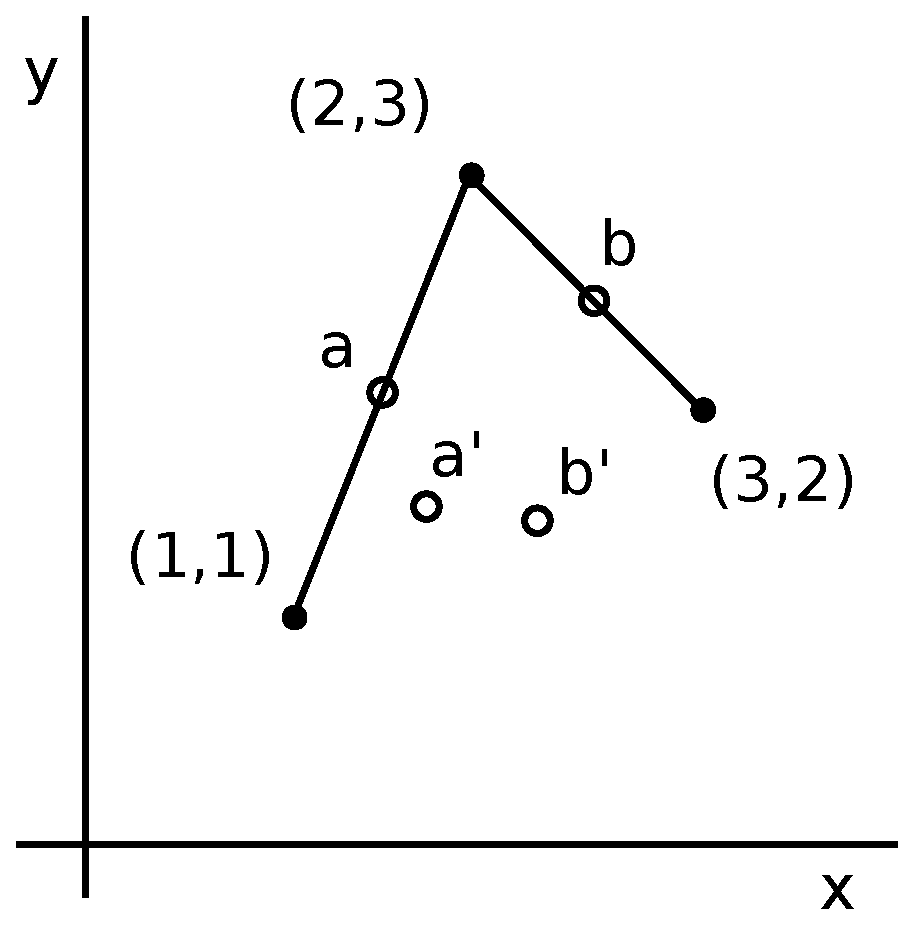
\includegraphics[width=\linewidth]{fig/interpolation-cartesian.eps}
    \caption{Cartesian Trajectory}
  \end{subfigure}
  \begin{subfigure}{0.45\linewidth}
    \def\svgwidth{\linewidth}
    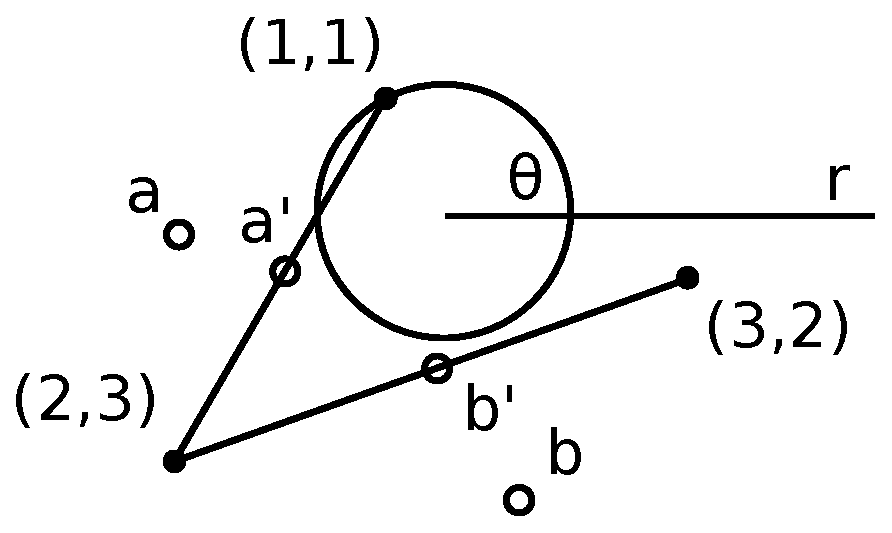
\includegraphics[width=\linewidth]{fig/interpolation-radial.eps}
    \caption{Radial Trajectory}
  \end{subfigure}
  \caption{Effect of the inner product on spatial geometry}
  \label{figure:cartesian-radial}
\end{figure}



\section{Information Theory}
\label{section:information-theory}

Shannon's information theory \cite{shannon1948mathematical}, though originally aimed at providing a theoretical foundation to signal processing and communication, has become foundational in all aspects regarding information.  According to information theory, the amount of information in a signal can be thought of as the amount of surprise at seeing a given quantity in that signal.  Put more simply, suppose you come in late to work one morning, and upon arriving into the office, your boss tells you about the weather. No information was gleaned from the conversation, since you already knew the weather from being outside.  If instead, upon entering the office late, your boss fires you, you would be very surprised, learning something unexpected, and gaining a lot of information.

\subsection{Entropy}
\label{subsection:entropy}

Though a concept originally borrowed from statistical physics that represents the amount of disorder in a system \cite{boltzmann1970weitere}, entropy can be applied to any probability distribution.  If applied to a discrete signal of symbols, it can be used to represent the amount of information of the signal (equation \ref{equation:entropy}), by taking it over the probabilities of each symbol $s$ of the alphabet $A$.

\begin{equation}
  \label{equation:entropy}
  H(s) = - \sum_{s \in A} p(s) \log_2 p(s)
\end{equation}

\subsection{Information Content}
\label{subsection:information-content}

Though entropy is useful in describing the quantity of information of a whole signal, to find the information content $h(s)$ of a single symbol $s$ in an alphabet, one must use equation \ref{equation:information-content} below. Since some symbols are less likely to occur than others, observing them gives more information than more likely ones, which is reflected here.

\begin{equation}
  \label{equation:information-content}
  h(s) = - \log_2 p(s)
\end{equation}

Whereas information content looks at a symbol in isolation, conditional entropy looks at symbols in pairs.  Conditional entropy is equivalent to the information content of a symbol, given that another symbol is known.  If we are referring to a stream of symbols, the conditional entropy would be the information content of a symbol given that we just saw the previous symbol.

\begin{equation}
  \label{equation:conditional-entropy}
  H(s|t) = -\log_2 p(s|t)
\end{equation}



\section{Information Dynamics of Thinking}
\label{section:idyot}

Cognitive architecture blending information theory and conceptual spaces.

\subsection{Boundary Entropy Segmentation}
\label{subsection:boundary-entropy-segmentation}

In natural language processing, n-gram models are often employed to track the frequency of chains of symbols in a given signal.  For instance, if examining textual data, a unigram model would count the frequency of individual words, whereas a bigram model would track the frequency of pairs of words.  It is clear that one can then utilize the information content measure on a unigram model and the conditional entropy measure on the bigram model in order to quantify the amount of information in that model. \cite{sproat1996stochastic}

\subsection{Sequential Memory}
\label{subsection:sequential-memory}

The sequential memory in IDyOT is represented as a hierarchy of chains of symbols. As the agent perceives a continuous stream of perception from the environment, it first discretizes that stream into moments, and links those discretized percepts as symbols in an ever-growing chain.  By examining time-varying information-theoretic properties of this chain, it can be chunked into a series of segments composed of a sequence of symbols.  This segment can then be abstracted by a representative symbol in the superior layer and can be said to subsume the inferior segment.  This process is done recursively until no more abstraction can be performed.

\subsection{Spectral Representations of Meaning}
\label{subsection:semantic-spectral-representation}

\subsection{Semantic Memory}
\label{subsection:semantic-memory}

If the sequential memory can be though of as how concepts relate to eachother over time, semantic memory can be thought of as how those concepts relate to eachother outside of time.  In IDyOT this is modeled using conceptual spaces.  At any given layer of abstraction in the sequential memory, there is a "parallel" semantic space for the symbols of that layer.  This allow us to think of a segment of symbols in sequential memory as a trajectory of concepts in semantic memory.  By looking at a spectral representation of this trajectory, the time-varying properties of the segment are removed, and this spectral representation can be thought of as an abstraction of the segment, and therefore as the abstracted symbol in the superior layer of the sequential memory.


\chapter{Theory \& Implementation}
\include{tex/theory-implementation/theory}
\section{Abstraction}
\label{section:abstraction}

When a segment is produced in the segmentation process, it is abstracted to a single symbol in the superordinate abstraction layer.  Since each dimension is composed of both an alphabet of symbols and a conceptual space in which those symbols live, a memory sequence is at once a segment of symbols in the sequential memory as well as a trajectory through the corresponding conceptual space in the semantic memory \citep{wiggins2019learning}. Since here we will utilize the formalism of finite-dimensional Hilbert spaces to model conceptual spaces, this trajectory corresponds to a time-parametric curve in a high-dimensional space.

\subsection{Fourier Transform}
\label{section:fourier-transform}

In the abstraction process, we would like to produce a spectral representation of a segment.  Here, we will apply the discrete Fourier transform (DFT) operator \citep{cooley1965algorithm} to the discrete trajectory (see equation \ref{equation:discrete-fourier-transform}), taking it from the time-domain $n$ to the frequency-domain $k$.  Though there are other spectral operators, there is evidence, especially in the auditory domain, that the brain operates on frequency transformations of time-varying signals from the Organ of Corti \citep{moore2012introduction}, and so it is employed here.  

\begin{equation}
  \label{equation:discrete-fourier-transform}
  \mathcal{F}_D [x_n] = X_k = \sum_{n=0}^{N-1} x_n e^{-\frac{i 2 \pi}{N} kn}
\end{equation}

By taking the Fourier transform (equation \ref{equation:fourier-transform}) of a time-varying signal $f(t)$, we produce the frequency-domain signal $F(\xi)$ for each orthogonal frequency.  So by taking the Fourier transform of a curve in a Hilbert space, we end up with a spectral representation of that curve.  The abstraction process will then consist of taking the Fourier transform of a trajectory through a Hilbert space, and then viewing the resulting frequency-domain signal as a point in the superordinate space.

\begin{equation}
  \label{equation:fourier-transform}
  \mathcal{F} [f(t)] = F(\xi) = \int_{-\infty}^\infty f(t) e^{-i 2 \pi \xi t} dt
\end{equation}

\subsection{Tensor Rank Promotion}
\label{section:tensor-rank-promotion}

The Fourier transform is an integral operator on Hilbert spaces \citep{kennedy2013hilbert}.  Since operators, by definition, take a function as input and produce a function as output, when thinking in terms of finite-dimensional Hilbert spaces, an operator will take the input from one domain to another, but will not change the shape of that input.  For example, if each point is represented as a vector, a sequence of those points would be a vector of vectors, i.e. a matrix.  Since we view the result of the Fourier transform as a point in the superordinate space, in our example, the point is now represented as a matrix.  Therefore, the result of abstracting a trajectory of points in a subordinate layer is a point in the superordinate space with one higher rank.  Hence, each level of abstraction promotes the rank of its constituent tensors by one. 

To clarify the first few stages of this process, consider Figure \ref{figure:tensor-rank-promotion}. The \textit{Element} row represents the constituent elements of layer $\alpha$.  The \textit{Trajectory} row strings those elements together, and the \textit{Spectral} row shows the shape of the spectral representation of that trajectory after the Fourier transform.  This spectral representation then becomes the constituent element of the superordinate abstraction layer $\alpha+1$.

We begin at the base abstraction layer with a space filled with the raw discrete scalar signal values for each moment of time.  By lining up these values and taking their Fourier transform, the resulting spectral representation is a vector.  This spectral representation is placed into the $\alpha=1$ abstraction layer, whose space is filled with points representing the frequencies of a signal of a short moment of time.  These points are vectors (rank 1 tensors) that, when strung together into a trajectory, form a matrix.  By taking the Fourier transform of this matrix and viewing the result as a point in the superordinate abstraction layer, that upper layer is now composed of points represented as matrices (rank 2 tensors).  Again, we string these points together as a trajectory, but now forming a cube.  By taking the Fourier transform, and viewing it as a point in the superordinate layer, that layer is now composed of points represented as cubes (rank 3 tensors). Repeating this process, we then get hypercubes of increasing rank at each layer of abstraction.  In this manner, the rank of a representative tensor increases by one for each layer of abstraction.

Unfortunately, this leads to an exponential explosion in the number of elements constituting a point in a given layer.  Formally, the number of elements is $r^\alpha$, where $r$ is the resolution of interpolation (see section \ref{section:interpolation}), and $\alpha$ is the level of abstraction.  Though this is not a problem in theory, it has consequences in terms of implementation.

\begin{figure}
  \centering
  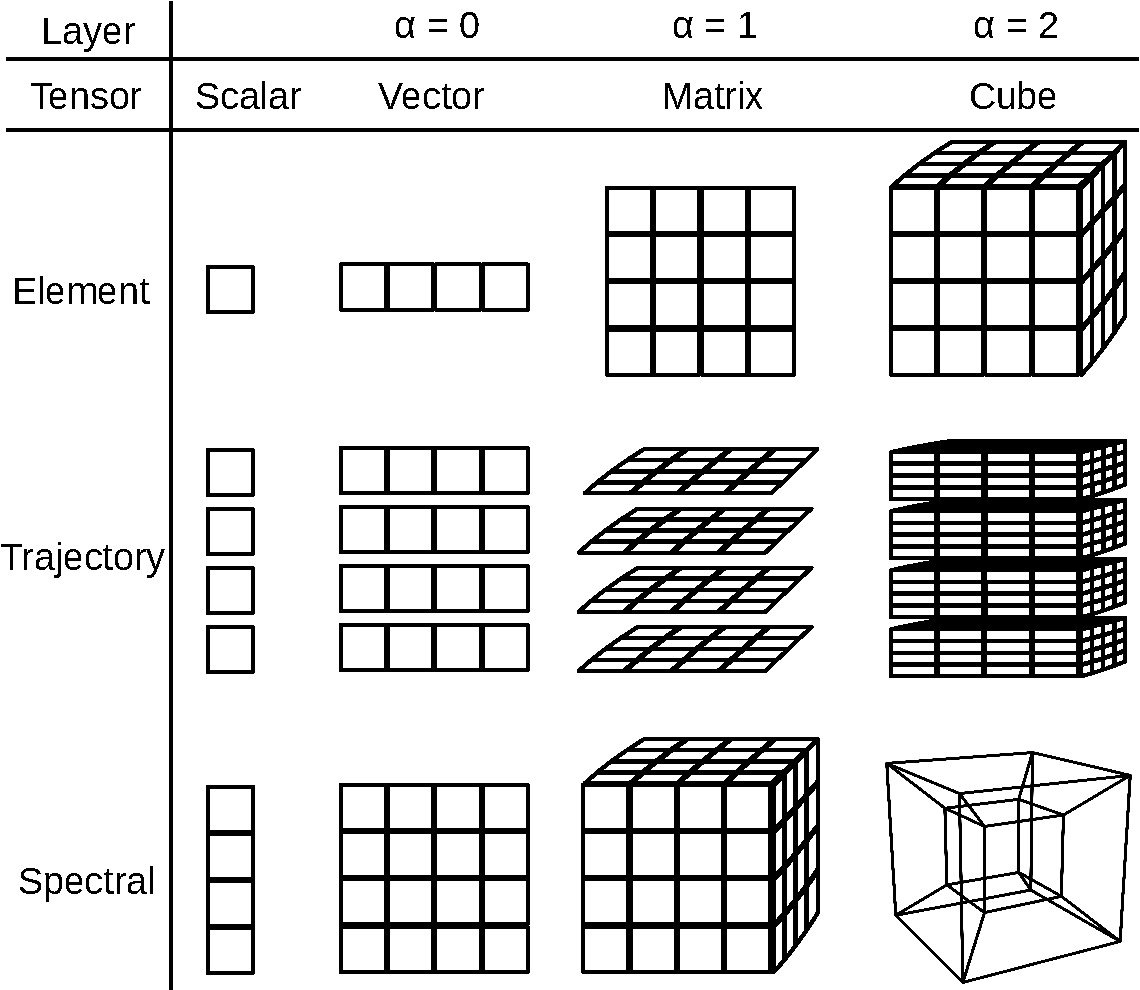
\includegraphics[width=\linewidth]{fig/tensor-rank-promotion.pdf}
  \caption{An illustration of tensor rank promotion for the first 4 levels of abstraction, using an interpolation resolution $r = 4$.  }
  \label{figure:tensor-rank-promotion}
\end{figure}

\subsection{Element-wise Independence}
\label{section:elementwise-independence}

When performing the Fourier transform on a tensor of any rank, it should be noted that each component in the tensor is independent from every other component.  Though this is not necessarily true of tensors in general, due to the particular hierarchical construction of these spaces by means of the DFT, each component is decoupled from the rest.  Starting at the bottom, the time-domain sound signal is transformed into a frequency-domain signal of coefficients in independent frequency bins.  It is this independence that allows us to represent the short-term frequency signal as a point with those frequency bins as dimensions.  Performing the DFT on the trajectory of frequency vectors results in independent frequency bins filled with vectors that possess independent entries, meaning all elements are independent one another.

Hierarchically performing the DFT at each abstraction layer on tensors with independent elements results in higher rank tensors with independent elements.  This element-wise independence of the tensor means that the DFT should be taken element-wise -- that is, across the base "time" axis -- since all other cross-component terms would involve orthogonal dimensions.

\subsection{Frobenius Norm}
\label{section:frobenius-norm}

The norm chosen for this implementation is the Frobenius norm \citep{horn1990norms}.  This norm corresponds with the familiar Euclidian norm, but since we are operating more generally on tensors, and not just vectors, the Frobenius norm is employed instead.  This norm corresponds to a flat space where each dimension behaves linearly and equally in relation to the other dimensions.  The Frobenius norm is intuitive for visualizing the space, and so serves as a good norm to begin exploration.  Future research will investigate different inner products and their induced norms to impose different geometries on the representations.

\begin{equation}
  \label{equation:frobenius-norm}
  \|A\|_F = \sqrt{\sum_{i=1}^m \sum_{j=1}^n |a_{ij}|^2}
\end{equation}

In equation \ref{equation:frobenius-norm}, the Frobenius norm is shown for a matrix.  One can then imagine that for a cube, there would be three summations, four summations for a hypercube, and so on.  Therefore, the Frobenius norm comes to be a sum over each element of the tensor.

\section{Segmentation}

Segmentation is the process of dividing an input stream into discrete chunks according to a difference function.

\subsection{Difference Function}
The difference function operates on the stream of symbols entering a given dimension and decides where segments begin and end.  Though there are a variety of ways in which to determine where to cut in this chain of symbols, here we will look at their information-theoretic properties to determine a meaningful cut. Primarily, we will look at moving entropy of the signal.  If the entropy rises, then a cut should be a made, marking the end of the current segment and the beginning of a new one.

Since entropy represents the amount of uncertainty at what comes next, it makes sense that a jump in entropy would mark the beginning of a new segment.  For instance, at the beginning of a sentence, entropy is high because the listener has little idea what the speaker will say next. As the sentence proceeds, the speaker will be better able to predict what comes next, meaning entropy is decreasing until the end of the sentences.  Once the sentence is finished, the listener again is less sure what will come next, and so entropy rises.  Therefore, at this rise in entropy, we would make a cut, resulting in a segment naturally representing the sentence just spoken.

This segmentation process results in two problems stemming from the two types of sparsity inherent in the segmentation and subsequent abstraction.

\subsection{Symbol Sparsity}
The first kind of sparsity arises from the length of the segment produced in the segmentation process.  Since the abstraction of the segment is its spectral transform, and we use the Discrete Fourier Transform (see section ?) to find the representative symbol in the superior abstraction layer, we run into precision problems due to the uncertainty principle of signal sparsity.  When performing a DFT, the signal precision is limited by the number of non-zero coefficients in either the time or frequency domain.  Therefore, if the number of symbols in a given segment is small, its spectral representation will be imprecise.  Therefore, it is necessary to perform interpolation (see section ?) to fill out the signal, so that high precision is maintained in the spectral transformation.

\subsection{Content Sparsity}
The second kind of sparsity is due to the nature of the symbol contents.  Since in the case of audio perception, the content of a symbol is a high-dimensional tensor of complex coefficients, not only are the possible values of each dimension uncountably infinite, there are a high number of uncountably infinite dimensions for each symbol.  Therefore, it is incredibly unlikely that any two symbols have exactly the same value for every dimension in the conceptual space in which they live.  

This poses a problem for determining the entropy and information content of symbols, which rely on the probability of a symbol.  If every symbol is unique, in the limit, the probability of seeing one in the signal is 0, meaning the entropy and information content each symbol in the signal would be 0. Really, the the probability of a unique event is meaningless, and therefore, even talking about its entropy is also meaningless.  

Though the space in which the symbols live is so sparse, we would still like to say that if two symbols are close enough together, for all intents and purposes (intensive porpoises), they are the same symbol.  This is accomplished through categorization (see section ?), where a label is attached to each symbol according to its category.  If two symbols have the same label, then they are equal, even though they may have different contents, that is, different values in their complex tensors.

\subsection{Symbol Generation}
When a segment is cut from the stream of symbols in a given dimension, a new symbol is generated that represents that segment in the superior abstraction layer.  At least in the case of all dimensions supervenient on audio perception, this means that the abstracted symbol is the spectral transformation of the segment.

\section{Categorization}

\subsection{Information Content Reduction Criterion} 
Since the goal of an IDyOT is to be as information-efficient as possible in its representation of concepts, the primary way to do this is categorize two different symbols together if they lead to an overall reduction in information content of the space.

However, if this reduction by information content measure was the only method used to determine categories, there would be nothing to stop all symbols from being categorized together.  If all the symbols are the same the information content is maximally reduced, but the result is a meaningless stream of monotony.  Obviously, this is unrealistic and undesirable.

\subsection{Categorical Convexity Criterion}
To push back against the reduction by information content is the categorical convexity criterion.  In section (?) we saw that categories in conceptual spaces are convex regions of the space, which translates to an infininite-dimensional hyperellipsoid in the corresponding Hilbert space.  What the convexity criterion guarantees is that for any two symbols in a given category, there is no symbol from a different category between those two symbols.

\subsection{Betweenness Relation}
Though this criterion is simple in formulation, the definition of what "between" actually means can vary greatly depending on the space in question.  Even when the space is unidimensional, the definition of between is somewhat arbitrary.  For instance, take the space that is wrapped aorund a circle.  Any point is between any other two points, depending on which direction around the circle you move.  Things get even less clear when moving into higher dimensions, where oftentimes, only a partial ordering is possible.

Therefore, instead of looking at betweenness at all, we instead incrementally build up categories by way of an inclusion radius around each point.  If another point falls within the inclusion radius, those poiints are categorized together.  In this way, we can ensure that ther eis never an interloper in a category, since if it was intruding on the region of the category, it would already be a member.

\subsection{Other Categorization Schemes} 
Chinese Restaurant Process is a nonparametric bayesian method that allows for unbounded clustering of new points in a space. Since for any given space, the number of "natural" categories is unknown, or perhaps unbounded, it makes sense to use a process that has the ability to add more categories as more data is seen in a given space, in the same way that humans are able to see more nuance the more trained they are in a given subject.

Locality-Sensitive Hashing allows for only a portion of the space to be searched for candidate categories.  Since points are only categorized together when they are close to eachother, there is no need to examine distant points as candidates.  Locality-sensitive hashing allows us to quickly determine what symbols are similar to a target symbol, and check if they should be categorized together.  This is the same as how humans are able to immediately sense similarity, though may require closer inspection to see if two subjects are actually of the same kind.


\section{Interpolation}
\label{section:interpolation}

When talking about trajectories through conceptual spaces, we refer to interpolation as the use of representative virtual points to perform the abstraction process instead of the actual values of the sequence.  Since we formalized semantic spaces as Hilbert spaces, we can analogously talk about drawing a time-parametric regression curve through points in the space.  Hence, the process of interpolation is simply sampling from a regression.

\subsection{Signal Sparsity}
\label{section:signal-sparsity}

As discussed in section \ref{section:symbol-sparsity}, interpolation is necessary to deal with symbol sparsity in a given segment.  To reiterate, this problem arises due to the use of the DFT in the abstraction process.  Since the precision of the transform is determined by the number of non-zero coefficients describing that signal, if the segmentation process results in a relatively short segment, the number of coefficients will be small, and the resulting transformation imprecise.  The way to deal with this imprecision is fill in coefficients such that the transform of the signal accurately represents the original signal, thereby producing a higher precision transform.  This is valid because we can think of the sparse signal as a sequence of samples from a function, and by regressing on those samples, we can obtain an approximate, but representative function of that segment.

\subsection{Hilbert Space Isomorphism}
\label{section:hilbert-space-isomorphism}

One fundamental aspect of Hilbert spaces is that all spaces of the same number of dimensions, even infinite, are isomorphic to all other Hilbert spaces of the same number of dimensions \citep{kennedy2013hilbert}.  Since we are using finite-dimensional spaces, to allow comparison between two points, we need their representative tensors to not only be of the same rank, but for each rank of the tensor to be the same size, so that the compared points have an equal number of dimensions.  Put another way, all points of a given space must have the same shape: that of the space.

Here, the problem arises during segmentation.  Since each segment in a given abstraction layer can be of arbitrary length, but we want the spectral transformations of all segments in a subordinate space to land in a single superordinate space, the transformation of the each segment must be taken over the same number of points.  Interpolation allows us to infer a curve through the points of a segment and place the required number of virtual points on that curve such that all segments have the same number of virtual points.  Then by taking the Fourier transform of these virtual points, we can be assured that the resulting spectral representation has the exact shape required to land in the space of the superordinate abstraction layer.

\subsection{Regression Sampling}
\label{section:regression-sampling}

In order to realize this process, we first regress through the available points of a segment.  In order to regress through the points, each point is assigned an index according to its relative place in the trajectory, and regression is performed through that series.  It is important to maintain the relative "lengths" of each point in this trajectory, where the length corresponds to the length of the segment of which this point is a spectral transformation in the subordinate layer.  Since segments are likely to be of different lengths, in this way, points at higher abstraction layers still maintain a sense of their connection to the base layer's time domain, yet still being time-invariant.  By spreading the index of a giving point according to its length for regression, this sense of relative length is maintained.

With the points now arranged according to their relative lengths, regression can be performed. Though the proper regression technique is still open to future research, in this implementation, Gaussian process regression \citep{williams1996gaussian} is employed.  Once the regression curve is found, the number of points according to the resolution hyperparameter $r$ is taken at equal intervals from the curve.  These virtual points will then be used in the spectral transformation of the abstraction process.

It should be noted that the value used for the the actual points in the regression are not of the points themselves, but rather of the centroid of the category that each point belongs to.  Therefore, when performing the regression, we are drawing a curve through categories instead of drawing a curve through instances.  This has the effect of making the spectral representations of similar trajectories consistent, thereby allowing them to land in the same region in the superordinate layer.

\subsection{Gaussian Process Regression}
\label{subsection:gaussian-process-regression}

One method for creating a smooth curve through these points is Gaussian process regression \citep{williams1996gaussian}.  By thinking of a sequence of points of a trajectory as a being drawn from a multivariate Gaussian distribution, we can think of a distribution of functions, i.e. a process, through those points.  The expectation of this process is the maximum a posteriori (MAP) function of the distribution, resulting in the highest likelihood trajectory through a sequence of points.  This method automatically avoids problems of overfitting inherent in higher-order transformation linear regression methods, though has the problem being prohibitively computationally expensive for a large number of points.  Fortunately, in this implementation the number of points is equal to the resolution of interpolation, which is quite small.

By utilizing the squared exponential kernel for Gaussian regression, the resulting trajectory will not only by the MAP curve, but also infinitely differentiable, meaning that it is maximially smooth.  This smoothness pays dividends when taking the Fourier transform of the trajectory, as the less smooth a sampled signal is, the larger the amplitude of high frequency artifacts of the Fourier transform become. We would like to avoid these artifacts, making this method of regression ideal for an interpolated spectral representation.

%\subsection{Trajectory Geometry}
%Though interpolation is necessary primarily to deal with problems mentioned above, it is also the main vehicle in which the geometry of the conceptual space imposes on the path of the trajectory of symbols.  Since in the Information Dynamics of Thinking, the interpretation of any space is determined by its inner product, we need to interpolate through that space in order to see the geometry.
%For instance, suppose we have three 2D symbols of which we want to draw a trajectory through. Consider two different spaces for conceiving those points: Cartesian (x, y) and Radial (r, $\theta$). Suppose we take the DFT of three points, i.e. as a trajectory without interpolation, in each of the two spaces.  Since the values of each point are exactly the same for both spaces, when examining the transform, there would be no way to tell which space it came from.  If instead we draw lines through the points and interpolate before taking the transform, we see clearly that the interpolated points differ between the two spaces, and so the transform of each trajectory will also be different.  In this way, the information about the geometry of the space can have an effect on the abstraction of the trajectory in that space.




\chapter{Empirical Analysis}
\include{tex/empirical-analysis/methods}
\section{Methodology}
\label{section:methodology}

\subsection{Parameterization}
\label{section:parameterization}

The parameterization of the implementation comes from two parameters: the resolution of interpolation $r$, and the initial radii $\rho_0$ of a category for each abstraction layer.  The resolution of interpolation is set to equal the sample window size used to slice the waveform, resulting in each rank of the tensor to be the same size at any given level.  Though we expect that a larger resolution will result in semantically richer categories in the higher levels, the exponential explosion in the size of the representative tensor, due to tensor rank promotion (see section \ref{section:tensor-rank-promotion}), results in exponentially increasing memory requirements (see table \ref{table:memory-requirements}). This limits the resolution to $r=16$ samples in our implementation.  However, it was found that below a certain resolution, the results are somewhat similar.  For instance, a 32-sample resolution behaves similarly to the 16-sample resolution, while having significantly higher processing and memory requirements.

\begin{table}
\centering
\begin{tabular}{@{}lllll@{}}
  \toprule
  Resolution $r$ & Layer $\alpha = 0$ & Layer $\alpha = 1$ & Layer $\alpha = 2$ & Layer $\alpha = 3$ \\
  \midrule
  16 & 0.25 KB & 4 KB & 64 KB & 1 MB \\
  32 & 0.5 KB & 16 KB & 512 KB & 16 MB \\
  64 & 1 KB & 64 KB & 4 MB & 268 MB \\
  128 & 2 KB & 262 KB & 34 MB & 4.3 GB \\
  \bottomrule
\end{tabular}
\caption{Memory Requirements for a single category with elements composed of 128-bit complex numbers}
\label{table:memory-requirements}
\end{table}

The initial radius $\rho_0$ for a new category in a given dimension has the largest effect on categorization within that dimension, and therefore also affects the segmentation of that layer.  Though the adaptive categorization method will alter the category volume according to its members, the initial radius will determine how willing a dimension as a whole is to categorize new instances.  If this initial radius is too small, then nothing will be categorized, and therefore nothing can be segmented.  If it is too large, then instances that should not be categorized together will be.  Due to the exponential growth in the number of elements in a tensor at each level, the initial radius parameters also grow exponentially.  Specifically, at zero-indexed abstraction level $\alpha$, the initial radius was manually set to $\rho_0 = 10^{\alpha}$.

\subsection{Data}
\label{section:data}

In order to evaluate the implementation on human speech, the TIMIT corpus \citep{garofolo1993darpa} was used.  This dataset has a large variety of American accents speaking a specific set of nonsense phrases that is meant to be used for natural language processing purposes.  Though having a large variety of speakers on which to train in order to diversify the semantic memory is useful, more importantly, each speech clip in the dataset is accompanied by annotations connecting words and syllables to a specific sample in the clip.  This allows us to compare the annotations and spectrogram of a clip with the categories of each layer in one unified visualization.  This allows us to examine if, for instance, categories at higher levels are associated with certain words or syllables.  

Since the word and syllable annotations mark qualitavely different sounds, these boundaries can be compared with the resulting categories at each level of abstraction to investigate if category boundaries align with word or syllable boundaries. If they do consistently, then this would be confirmation that the segmentation, categorization, and abstraction processes are working as envisioned in the theory. 

\subsection{Experiments}
\label{section:experiments}

The IDyOT was trained on a 10-clip set from a single speaker, ranging from 1.5 seconds to 4 seconds, with most clips being around 3 seconds.  With a resolution of $r=16$ samples, this test set results in over 26000 distinct slices of speech to be analyzed.  Though, theoretically the maximum abstraction layer is unknown, but likely quite large, here it was capped at the fourth level $\alpha = 3$ due to processing and memory limitations.  The resulting categorization in semantic memory was then used to seed a sequential memory from a single clip of the same speaker.

Here the speaker is a young woman from somewhere in New England, perhaps a borough of New York or Boston, identified as TRAIN-DR1-FCJF0 in the TIMIT corpus.  After training on all available audio for this speaker, the SA1 clip was used for analysis, which has the same speaker reading the nonsense line: "She had your dark suit in greasy wash water all year."

In an earlier iteration of the implementation, a larger 53-clip training set containing a variety of different accents and sentences was used to train the IDyOT, but the resulting visualization (see section \ref{section:results}) was not qualitatively different than the 10-clip set, while actually being more difficult to inspect due to the increased number of categories from the larger set.  Therefore, the 10-clip training set was used for visualization.

\section{Results}

\subsection{Sequential Memory Category Flow}

\subsection{Semantic Memory Spatial Plot}

\subsection{Categorical Consistency Matrix}


\chapter{Evaluation \& Discussion}
\section{Discussion}
\label{section:discussion}

\subsection{Addressing Categorical Inconsistencies}
\label{section:addressing-categorical-inconsistencies}

Though the category similarity matrix confirms that some similar-sounding syllables are either categorized together or at least near each other in the space, there are also confusing portions.  For instance, the entire word 'water' is categorized into a few very similar categories.  At higher levels of abstraction than seen here, one might expect that whole words would compose a single category, but since at abstraction level 3 we seem to be still mostly categorizing syllables and diphtongs, we would not expect the entire word to be one category.

This over-categorization may be due to two issues.  The first may be that the categorization is too eager in this location, resulting in different points being grouped together that should not be.  Though a significant amount of tuning was performed to find good initial radii for each layer, it's possible that a lower radius at this level would result in a more intuitive categorization for this particular region.

On the other hand, it may instead be due to the segmentation scheme employed in this implementation.  Here, we segment the stream at either a rise in entropy \textit{or} a rise in information content, resulting in numerous, relatively short segments.  Though there are a large number of segments, any given segment will not contain much information, by nature of its short length.  For a less eager segmentation, we could segment at a rise in just one of the measures.  This would result in fewer but longer segments with more information per segment. Though there would be fewer resulting categories from this reduced scheme, each category would be richer in that it represents more information, and may result in categories that consistently represent full syllables at this level of abstraction.

\subsection{Meaningful Categorizations}
\label{section:meaningful-categorizations}

That being said, though not perfect, we do observe the emergence of a few consistent categories that represent syllables at abstraction layer 3.  Since we also clearly see that similar trajectories are being categorized together in higher layers, it is a tenuous confirmation that the abstraction process as set forth in the theory behaves as intended.  We can see that even at a relatively low abstraction level 3, the hierarchical spectral representations of the speech signal are coalescing into categories that could be said to represent human speech sounds.  One could imagine, given a few more levels of abstraction and significantly more training, that the higher-level abstraction categories would become consistent, meaningful representations of the human speech signals they are learned from.

\subsection{Unified Approach to Perceptual Representation}
\label{section:unified-approach-to-perceptual-representation}

What makes these results exciting is not just that we are beginning to see the emergence of syllables as discrete categories, but the general applicability of this method.  Not only might we expect to see more complex elements of human speech such as words, sentences, and even syntax start emerge as categories in higher levels of abstraction, but the processes of segmentation, categorization, and abstraction are agnostic about the domain of the data in operation. That is, instead of using human speech signals as the raw input, another audio domain such as music could be used, as in IDyOM \citep{pearce2005construction}.  In general, just about any time-varying signal could be used instead.  Since other modes of perception such as vision can be modeled as time-varying signals, if consistent categories can be found for these human speech signals, perhaps semantically rich categories could be found for these other domains as well.  Doing so would uncover related semantics from different areas of perception, resulting in a more holistic coginitive architecture that ties in the multitude of domains of human experience.


\chapter{Conclusion}
\include{tex/conclusion/conclusion}
\section{Contributions}
\label{section:contributions}

There are a number of significant contributions from this thesis that move toward a formal implementation of the Information Dynamics of Thinking theory, which up until now, and not counting other IDyOT-like systems \citep{forth2016entraining}, was almost entirely a theoretical proposition.  Specifically, a significant portion of Chapter 3: Theory \& Implementation is work contributed by the author, though of course with guidance from the promoter and advisor, Prof. Dr. Dr. Geraint Wiggins.  A short review of specific contributions is presented in the following paragraph.  

Tensor rank promotion (section \ref{section:tensor-rank-promotion}) and element-wise independence (section \ref{section:elementwise-independence}) of the tensors produced in the abstraction process, though falling directly from the theory, were identified by the author. Though content sparsity was known prior in the theory, the problem of signal sparsity (section \ref{section:signal-sparsity}), in conjunction with the necessity for equal-shaped tensors falling from Hilbert space isopmorphism (section \ref{section:hilbert-space-isomorphism}) led to the need for interpolation (section \ref{section:interpolation}) and its proposed solution in regression sampling (section \ref{section:regression-sampling}).  In addition, the adaptive categorization (section \ref{section:adaptive-categories}) technique expanded on the idea of an inclusion radius and made it adaptive to the constituents of the category.

Beyond these theoretical contributions, this is the first, albeit limited, realized implementation of IDyOT that utilizes all three main processes: abstraction, segmentation, and categorization. As seen in the results, this is the first empirical analysis that spectral representations of meaning in the context of IDyOT, at least in human speech, can produce identifiable representations in a hierarchical manner.  This highly novel and general approach to perceptual representation could have far-reaching consequences, but here was the first empirical result that the whole theory might be viable.

\section{Limitations}

\section{Future Work}

\subsection{Inner Products}

\subsection{Spectral Projectors}


\appendix
\renewcommand{\chaptermark}[1]{\markboth{\MakeUppercase{\appendixname}\ \thechapter.\ #1}{}}
\chapter{Appendix} \label{App:AppendixA}
\addtocontents{toc}{\protect\setcounter{tocdepth}{0}}



\bibliographystyle{apacite}
\bibliography{thesis}

\end{document}
